\section{Question1}
\subsection{Problem:}
Consider the unique interpolating polynomial $p_{n}(x)$ of degree n or less that interpolates a
function f(x) at n + 1 equally spaced interpolation points \\
\begin{align*}
{x_0, x_{1}, x_{2}, \ldots , x_{n}}
\end{align*}
on an interval [a, b], taking $x_0$ = a and $x_n = b$. \\
Write a program to do the following: Use the Lagrange basis functions $l_{i}(x), i = 0, 1, 2,\ldots n$
on Pages 169-172 of the Lecture Notes to evaluate pn(x) at M + 1 equally spaced sampling
points \\
\begin{align*}
{y_0, y_1, y_2, \ldots , y_M},
\end{align*}
where y0 = a and yM = b, and where M is much larger than n. Estimate the maximum
interpolation error \\
\begin{align*}
max_{[a,b]}  |f(x) − p_{n}(x)|
\end{align*}
by computing the approximate maximum interpolation error \\
\begin{align*}
max_{0\le i \le M} |f(yi) − pn(yi)|
\end{align*}
Specifically, do the above for each of the following cases :
\begin{itemize}
    \item $f(x) = \sin(\pi x) , \text{on the interval} [−1, 1] , i.e., a = −1 \text{ and } b = 1)$
    \item $\frac{1}{1+x^2}$, on the interval [−2, 2]
    \item $\frac{1}{1+x^2}$, on the interval [−5, 5]
\end{itemize}

successively using n = 2, 4, 8, 16. In each case use M = 500. \\
For each of these 12 cases print the approximate maximum interpolation error. \\
Also, for each of the three functions f(x), give a graph that shows f(x) and the polynomials 
$p_{n}(x)$, n = 2, 4, 8, 16. \\
In addition, for the case $f(x) = \sin(\pi x)$ on the interval [−1, 1], use the Lagrange Interpolation
Theorem on Page 176 and the Table on Page 183 of the Lecture Notes to derive an upper
bound on the maximum interpolation error for n = 2, 4, 8, 16. Compare this upper bound to
the actual (approximate) maximum interpolation error found above.
Give a concise summary and discussion of your findings.

\subsection{Lagrange Interpolation}
The Lagrange Interpolation was carried out by using Python with Jupyter Notebook. 
Check out the full source code and presentation in directory: \textit{program/Problem\_1.ipynb}
Below is the main algorithm:
\begin{lstlisting}
def lagrange(f, listXi, listYi, n):
    def approximate(x):
        listLi = list()
        for i in range(n):
            Li = 1
            for j in range(n):
                if(j==i):
                    continue
                Li = Li * ((x - listXi[j]) / (listXi[i] - listXi[j]))
            listLi.append(Li)

        approx = 0
        for i in range(n):
            approx = approx + listLi[i] * listYi[i]
        return approx

    return approximate
\end{lstlisting}

To get the list of iteration and the list of points to be examined. The following 2 methods were used:

\begin{lstlisting}
def getListOfEvaluation(a, b, M):
    listInterpolation = list()
    fraction = (b - a)/M
    temp = a
    for i in range(M+1):
        listInterpolation.append(temp)
        temp += fraction
    return listInterpolation

def getListX(a, b, n):
    listX = list()
    fraction = (b - a)/n
    temp = a
    for i in range(n+1):
        listX.append(temp)
        temp += fraction
    return listX
\end{lstlisting}

After that, \textit{evaluatePerror()} will approximate the maximum error of the interpolation as following:

\begin{lstlisting}
def maxInterpolationError(f, realList, listP, numOfPoint):
    maxErr = 0
    for i in range(numOfPoint):
        err = abs(realList[i] - listP[i])
        if err > maxErr:
            maxErr = err

    return maxErr

def evaluatePerror(f, a, b, n, M):
    listX = getListX(a, b, n)
    iterList = getListOfEvaluation(a, b, M)
    Px = lagrange(f, listX, list(map(f, listX)), n)
    listP = list(map(Px, iterList))
    realList = list(map(f, iterList))
    numOfPoint = M + 1
    return maxInterpolationErrorNew(f, realList, listP, numOfPoint)
\end{lstlisting}

\newpage
\subsection{Function 1 $\sin (\pi x)$ on interval [-1, 1]}
The output is as followed:\\
\begin{centering}
    \includegraphics[scale=0.5]{p_1fSin_n2}\\
    \includegraphics[scale=0.5]{p_1fSin_n4}\\
    \includegraphics[scale=0.5]{p_1fSin_n8}\\
    \includegraphics[scale=0.5]{p_1fSin_n16}\\
\end{centering}

\newpage
\subsection{Function 2: $\frac{1}{1+x^2}$ on interval [-2, 2]}
The output is as followed:\\
\begin{centering}
    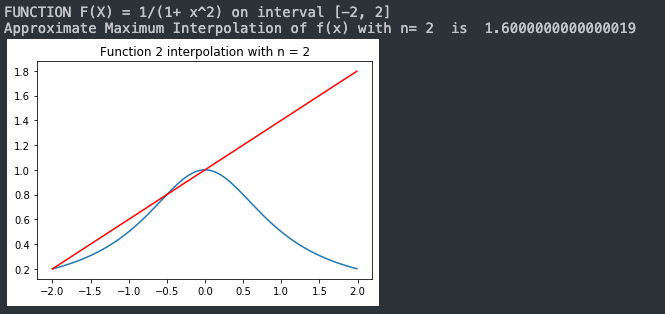
\includegraphics[scale=0.5]{p_1f2_n2}\\
    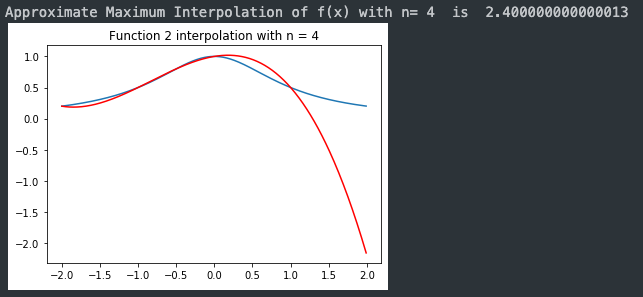
\includegraphics[scale=0.5]{p_1f2_n4}\\
    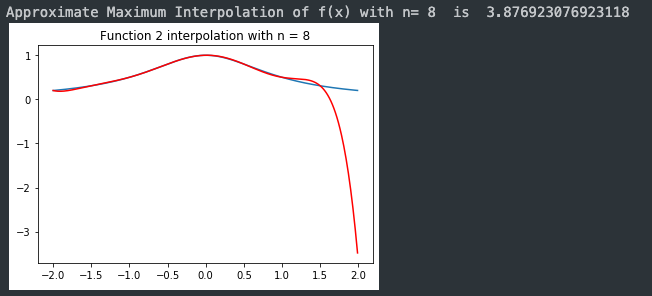
\includegraphics[scale=0.5]{p_1f2_n8}\\
    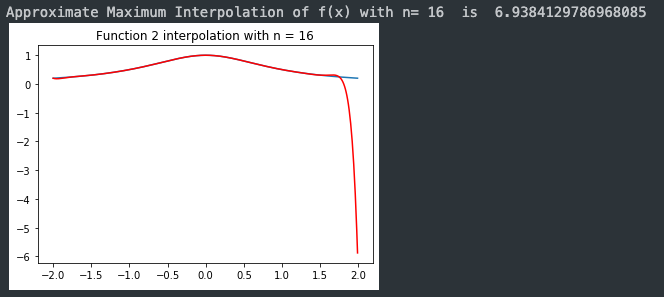
\includegraphics[scale=0.5]{p_1f2_n16}\\
\end{centering}

\newpage
\subsection{Function 3: $\frac{1}{1+x^2}$ on interval [-5, 5]}
The output is as followed:\\
\begin{centering}
    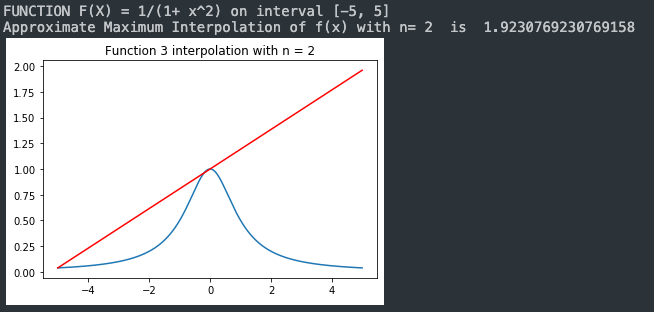
\includegraphics[scale=0.5]{p_1f3_n2}\\
    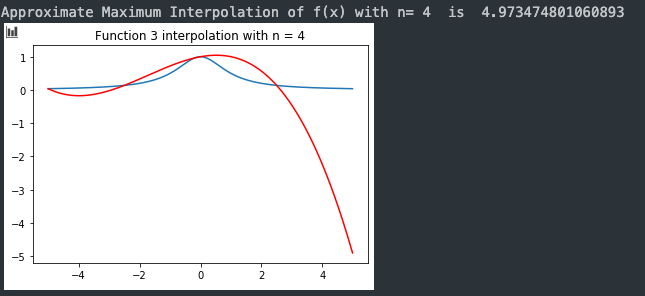
\includegraphics[scale=0.5]{p_1f3_n4}\\
    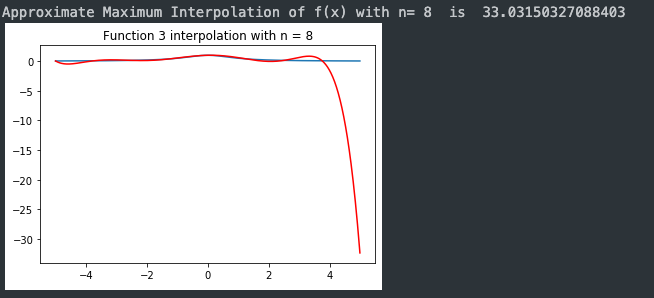
\includegraphics[scale=0.5]{p_1f3_n8}\\
    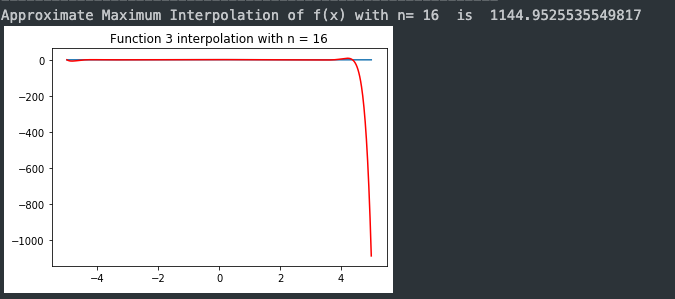
\includegraphics[scale=0.5]{p_1f3_n16}\\
\end{centering}

\newpage
\subsection{Summary:}
As observed, since the approximate maximum error could be increased when n increases, it can not be concluded that the more points (n) were examined to create the interpolating function, the smaller the error would be. However, the Lagrange interpolating function does a good job on interpolating the given function in term of shape.\\
Another conclusion would be interpolating a function by a high degree polynomial is not a good idea.
